\section{Control of underactuated robots}
The present section delves into the application of the strategy illustrated so far to the control of two examples of underactuated robots - the pendubot and the acrobot.
\subsection{Mathematical model}
The pendubot and the acrobot share the same dynamics of a 2R planar robot moving in the vertical plane. With reference to \cite{lanarioriolo}, which in turn quotes \cite{siciliano}, to describe these dynamics we introduce the system of differential equations:
\begin{equation}
    M(q) \ddot{q} + B \dot{q} + c(q, \dot{q}) + e(q) = u, \label{eq:dyn_robot}
\end{equation}
where $q = \begin{bmatrix} q_1 & q_2 \end{bmatrix}^\top$ is the vector of joint angles, $\dot{q}$ and $\ddot{q}$ are the joint velocity and acceleration, respectively, and $u = \begin{bmatrix} u_1 & u_2 \end{bmatrix}^\top$ is the control input. \\
Moreover, $M(q)$ is the inertia matrix:
\begin{equation*}
    M(q) = \begin{bmatrix}
        a_1 + 2a_2 c_2 & a_3 + a_2 c_2 \\
        a_3 + a_2 c_2 & a_3
    \end{bmatrix},
\end{equation*}
$B$ is the (positive definite) dissipation matrix: 
\begin{equation*}
    B = \begin{bmatrix}
        b_1 & 0 \\
        0 & b_2
    \end{bmatrix},
\end{equation*}
$c(q, \dot{q})$ is the Coriolis and centrifugal vector: 
\begin{equation*}
    c(q, \dot{q}) = \begin{bmatrix}
        a_2 s_2 \dot{q}_2 (\dot{q}_2 + 2 \dot{q}_1) \\
        a_2 s_2 \dot{q}_1^2
    \end{bmatrix},
\end{equation*}
and $e(q)$ is the gravity vector:
\begin{equation*}
    e(q) = \begin{bmatrix}
        a_4 s_1 + a_5 s_{12} \\
        a_5 s_{12}
    \end{bmatrix}.
\end{equation*}
Here, we use the compact notation:
\begin{align*}
    s_1 &= \sin(q_1), & c_1 &= \cos(q_1), \\
    s_2 &= \sin(q_2), & c_2 &= \cos(q_2), \\
    s_{12} &= \sin(q_1 + q_2), & c_{12} &= \cos(q_1 + q_2),
\end{align*}
and the (positive) constants:
\begin{align*}
    a_1 &= I_{1zz} + m_1 d_1^2 + I_{2zz} + m_2 (l_1^2 + d_2^2), \\
    a_2 &= m_2 l_1 d_2, \\
    a_3 &= I_{2zz} + m_2 d_2^2, \\
    a_4 &= g (m_1 d_1 + m_2 l_1), \\
    a_5 &= g m_2 d_2.
\end{align*}
\begin{figure}[H]
    \centering
    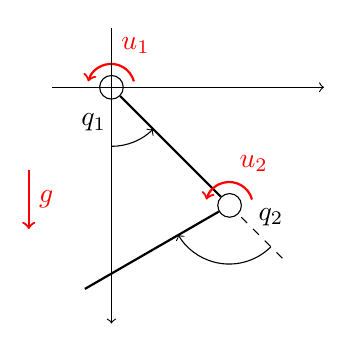
\begin{tikzpicture}[scale=1.5]
        \coordinate (O) at (0,0);
        \coordinate (A) at (1,-1);
        \coordinate (B) at (-0.225,-1.707);
        \coordinate (C) at (1.48,-1.48);
        
        \draw[thick] (O) -- (A) -- (B);
        \draw[dashed] (A) -- (C);
        
        \filldraw[white] (O) circle (0.1);
        \draw (O) circle (0.1);
        \filldraw[white] (A) circle (0.1);
        \draw (A) circle (0.1);
        
        \draw[->] (0,-0.5) arc[start angle=270, end angle=315, radius=0.5];
        \draw[->] (A) ++(0.35,-0.35) arc[start angle=315, end angle=210, radius=0.5];
        
        \node at (-0.15,-0.3) {$q_1$};
        \node at (1.35,-1.1) {$q_2$};
        
        \draw[red,->,thick] (O) ++(0.19,0.05) arc[start angle=15, end angle=165, radius=0.2] node[midway, above right] {$u_1$};
        \draw[red,->,thick] (A) ++(0.19,0.05) arc[start angle=15, end angle=165, radius=0.2] node[midway, above right] {$u_2$};
        
        \draw[red,->,thick] (-0.7,-0.7) -- ++(0,-0.5) node[midway, right] {$g$};
        
        \draw[->] (-0.5,0) -- (1.8,0);
        \draw[->] (0,0.5) -- (0,-2);
    \end{tikzpicture}
    \caption{Graphical representation of a 2R planar robot in the vertical plane.}
    \label{fig:robot}
\end{figure}
The only difference between the two robots lies in the actuation, since the only actuated joint of the pendubot is the “shoulder” (implying that $u_2 = 0$), while that of the acrobot is the “elbow”(therefore $u_1 = 0$).

\subsection{Control objective}
The equilibria of the robot are found by setting all the derivatives of the generalized coordinates to zero. Among these, the unforced ones are identified by solving the equation:
\begin{equation*}
    e(q) = 0,
\end{equation*}
which corresponds to the condition of balance of the gravity forces, yielding the four solutions:
\begin{equation*}
    q_{uu} = \begin{bmatrix} \pi \\ 0 \end{bmatrix}, \quad
    q_{ud} = \begin{bmatrix} \pi \\ \pi \end{bmatrix}, \quad
    q_{du} = \begin{bmatrix} 0 \\ \pi \end{bmatrix}, \quad
    q_{dd} = \begin{bmatrix} 0 \\ 0 \end{bmatrix}.
\end{equation*}

The control objective is to stabilize the robot in the upright position $q_{uu}$ with zero final velocity, starting from the initial conditions $q_0 = q_{dd}$ and $\dot{q}_0 = 0$. This is known as the \textit{swing-up problem}, and it is a challenging task due to the underactuation of the system, since the control input is constrained to the actuated joint, and the other joint is passive.

In addition, the control input is subject to the (component-wise) inequality constraint:
\begin{equation}
    u_{\text{min}} \leq u \leq u_{\text{max}}, \label{eq:input_constraints}
\end{equation}
to be intended as a saturation limit on the torque that can be applied to the actuated joint. Obviously, the input is also subject to the physical constraint $u_2 = 0$ for the pendubot and $u_1 = 0$ for the acrobot, and therefore $u_{\text{min}}$ must be non-positive and $u_{\text{max}}$ non-negative.

\subsection{Control strategy tailoring}
The control strategy illustrated so far can be adapted to the specific case of the pendubot and the acrobot by considering the following. 

\subsubsection{Dynamics}
First of all, we have to translate our nonlinear dynamics \ref{eq:dyn_robot} in terms of \ref{eq:dyn}. To this end, we define the state vector: 
\begin{equation*}
    x = \begin{bmatrix} x_1 & x_2 & x_3 & x_4 \end{bmatrix}^\top = \begin{bmatrix} q^\top & \dot{q}^\top \end{bmatrix}^\top.
\end{equation*}
As far as the control input is concerned, we use: 
\begin{equation*}
    u = \begin{bmatrix} u_1 & 0 \end{bmatrix}^\top
\end{equation*}
for the pendubot and: 
\begin{equation*}
    u = \begin{bmatrix} 0 & u_2 \end{bmatrix}^\top
\end{equation*}
for the acrobot. Therefore, the dynamics of the robot, rewritten in terms of \ref{eq:dyn}, are given by defining the $4\times1$ state transition function:
\begin{equation*}
    f(x, u) = \begin{bmatrix} x_3 \\ x_4 \\ M^{-1}(x)\left(-B\begin{bmatrix}x_3 \\ x_4\end{bmatrix} - c(x) - e(x) + u\right) \end{bmatrix}.
\end{equation*}

Finally, according to this new representation, the swing-up problem undergoes the following modifications:
\begin{itemize}
    \item the initial state is $x_0 = \begin{bmatrix} q_{dd}^\top & 0 & 0 \end{bmatrix}^\top$;
    \item the (final) reference state is $x^* = \begin{bmatrix} q_{uu}^\top & 0 & 0 \end{bmatrix}^\top$.
\end{itemize}

\subsubsection{Cost function}
Another important object to tailor is the cost function \ref{eq:cost}, and, for this purpose, a common and simple choice is to use quadratic functons. In particular, we select:
\begin{align*}
    l(x,u) &= (x-x^*)^\top P (x-x^*) + u^\top R u,\\
    l_f(x) &= (x-x^*)^\top P^N (x-x^*),
\end{align*}
where $P$, $R$ and $P^N$ are positive definite matrices. The choice of the cost function is fundamental, since it determines the behavior of the control law. In this case, in the spirit of our control objective, we choose $P$ and $P^N$ to penalize the deviation from the equilibrium position, as well as $R$ to weight the control effort. \\
In conclusion, the total cost function is modified accordingly:
\begin{gather*}
    J(x^0, U) = \sum_{i=0}^{N-1} (x^i-x^*)^\top P^i (x^i-x^*) + u^{i\top} R u^i \;+\;\\ +(x^N-x^*)^\top P^N (x^N-x^*).
\end{gather*}
Notice that, since $J$ is evaluated over the current control horizon, the weight matrix $P^i$ should change with each iteration to accomodate the slide of the final cost $P^N$. \\

\subsection{Simulations}
The current section is intended to present the results that we obtained. \\
The two closed loops, each consisting of the complete controller and one of the two robots (whose parameters are summarized in \ref{tab:parameters}), have been implemented and simulated in \textit{MATLAB R2024a}. \\
The experiments consist of running the code for a total time of $5$ seconds, with time steps of $T = 0.01$ seconds. The (receding) control horizon of the controller is set to $N = 300$, which corresponds to $3$ seconds. \\
We have also tested, for each robot, the three different methods for constraining the input, aiming to highlight their differences.

\begin{table}[H]
    \centering
    \renewcommand{\arraystretch}{1.2}
    \setlength{\tabcolsep}{10pt}
    \begin{tabular}{ccc}
    \toprule
    \textbf{Parameter} & \textbf{Symbol} & \textbf{Value} \\ \midrule
    Gravity & $g$       & 9.81 [\SI{}{\meter\per\second\squared}] \\
    Link length & $l$       & 0.5 [\SI{}{\meter}] \\
    Link mass & $m$       & 2 [\SI{}{\kilogram}] \\
    Link inertia & $I$       & $\frac{1}{12} m l^2 \, [\SI{}{\kilogram\meter\squared}]$ \\
    Link COM & $d$       & $\frac{l}{2} \, [\SI{}{\meter}]$ \\
    \bottomrule
    \end{tabular}
    \caption{Robot parameters}
    \label{tab:parameters}
\end{table}

\subsubsection{Pendubot}
Recall that the model of the pendubot is obtained by not actuating the second joint of the 2R vertical planar robot in Figure \ref{fig:robot}, i.e., by setting $u_2$ identically equal to zero. Meanwhile, the limits imposed on the actuated joint are $u_{\text{min}} = -\SI{5}{\newton\meter}$ and $u_{\text{max}} = \SI{5}{\newton\meter}$.

Figure \ref{fig:pendubot_traj} shows the trajectories of the pendubot under the three different constraining strategies: notice that, other than the case with no constraints, only the constrained quadratic programming method is able to stabilize the robot in the upright position (as illustrated also in Figure \ref{fig:pendubot_anim}). With the naive clamping approach, it is evident (especially at the beginning) that the control sequence is a sharply cut version of the unclamped sequence, which is not adequate to reach the goal; using the squashing function, the smoothing effect on the control curve is evident, the nonlinearity of which, however, puts the controller in a difficult position to find a useful control trajectory.

\end{multicols}
\begin{figure}[H]
    \centering
    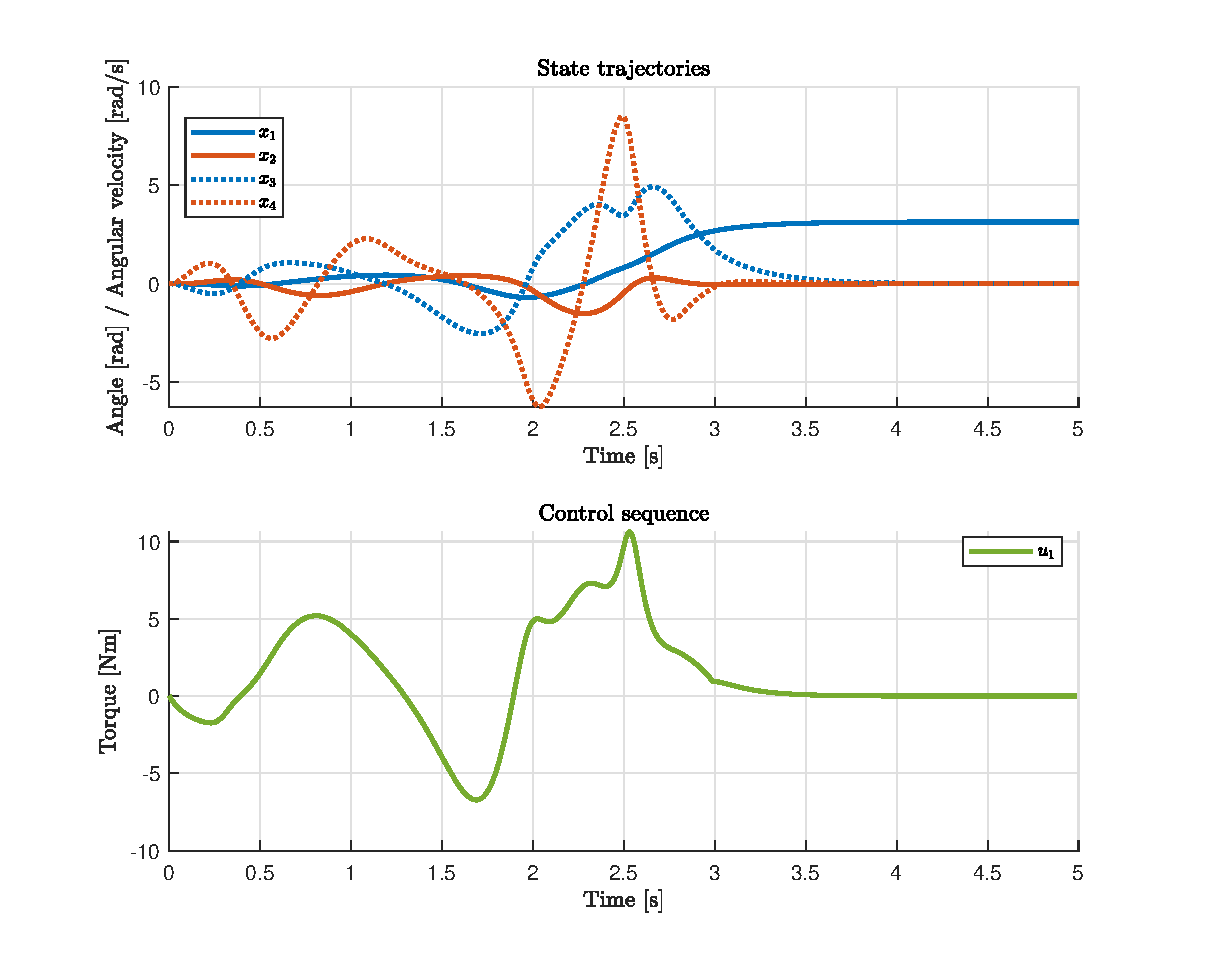
\includegraphics[width=0.4\textwidth]{assets/pendubot_traj.eps}
    \includegraphics[width=0.4\textwidth]{assets/pendubot_nc_traj.eps} \\
    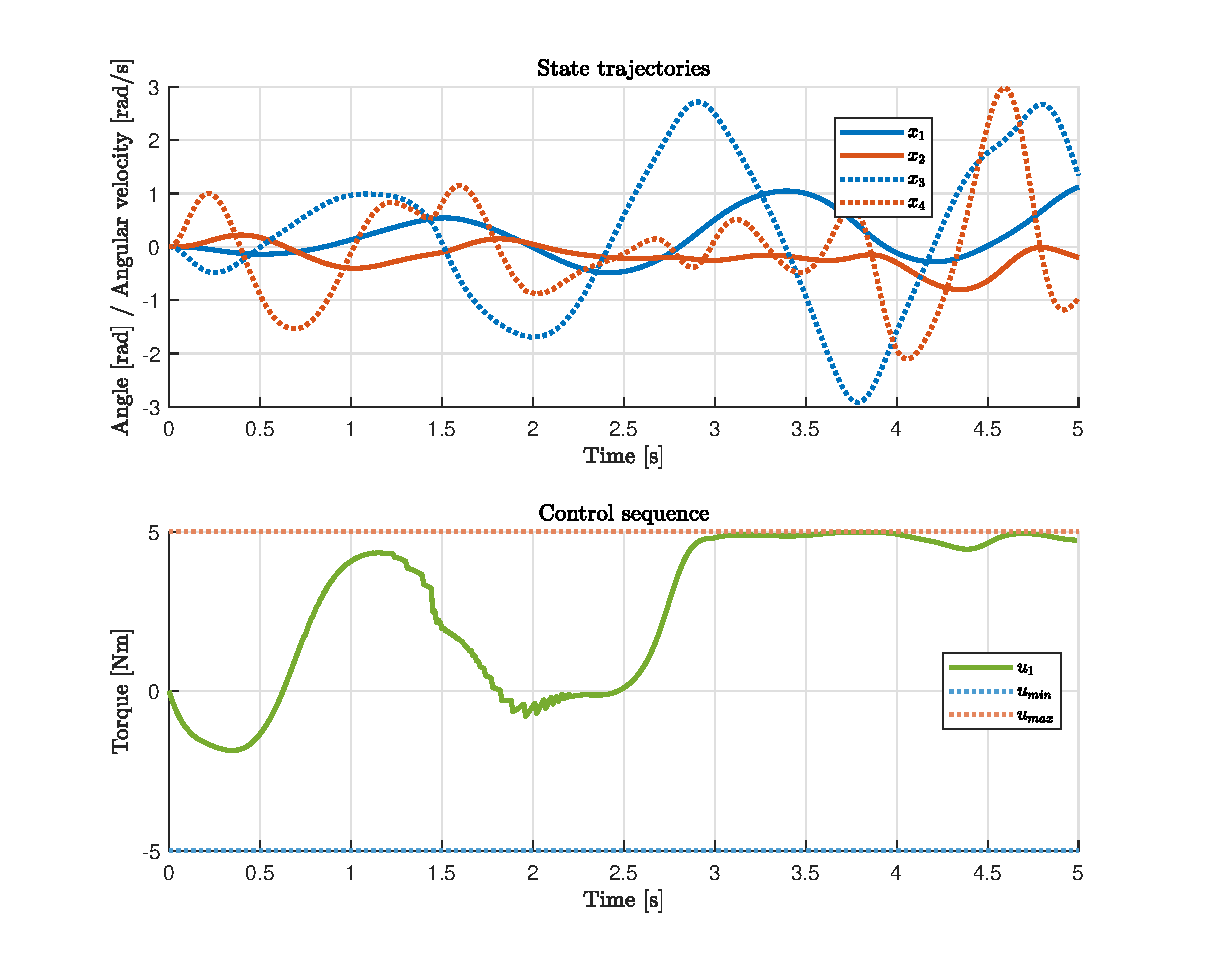
\includegraphics[width=0.4\textwidth]{assets/pendubot_sf_traj.eps}
    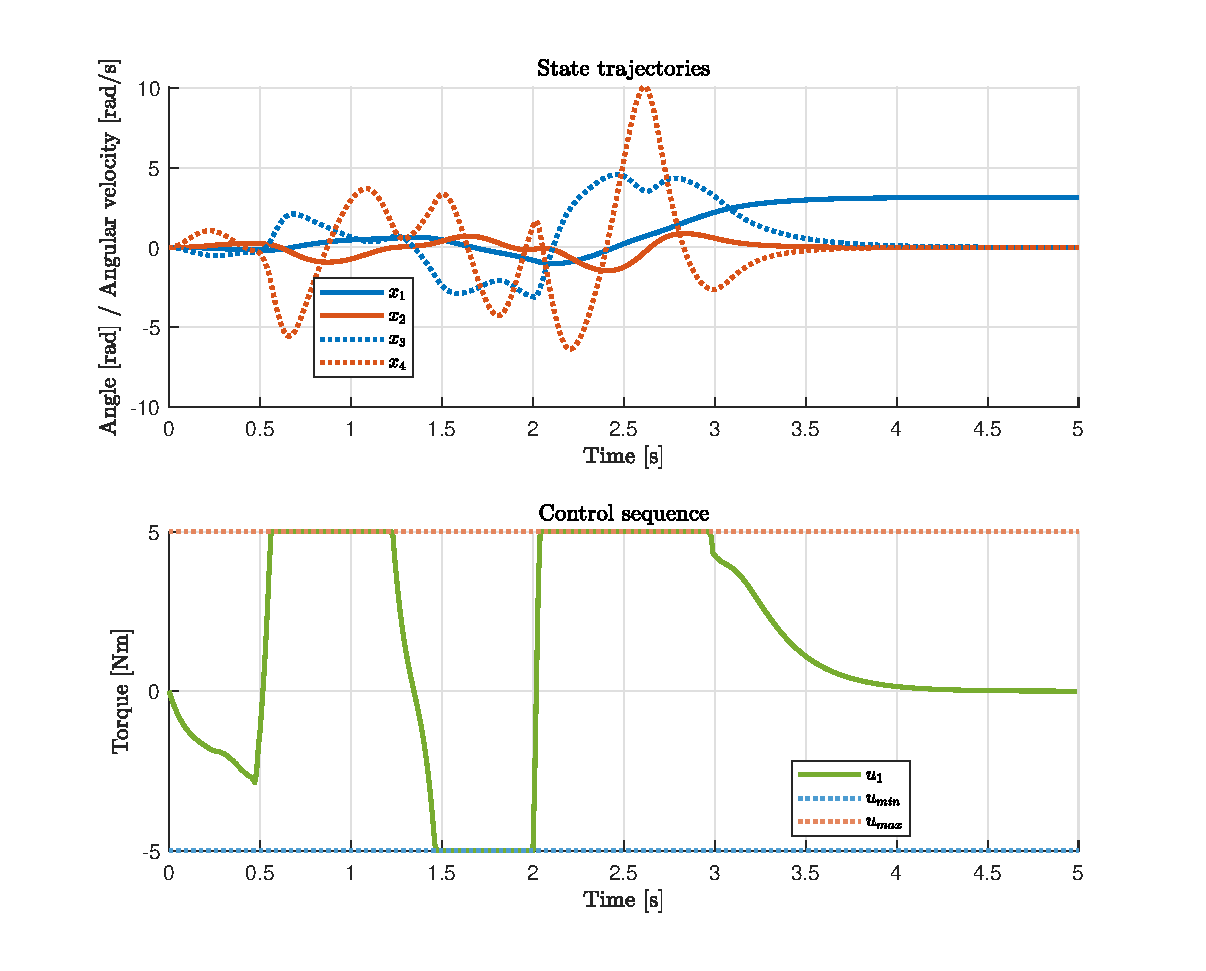
\includegraphics[width=0.4\textwidth]{assets/pendubot_qp_traj.eps}
    \caption{Trajectories of the pendubot under: no constraints (top left), naive clamping (top right), squashing function (bottom left), constrained quadratic programming (bottom right).}
    \label{fig:pendubot_traj}
\end{figure}

\begin{figure}[H]
    \centering
    \includegraphics[width=0.25\textwidth,trim={3cm 1cm 1cm 1cm},clip]{assets/pendubot_qp_anim_1.eps} \hspace*{-0.5cm}
    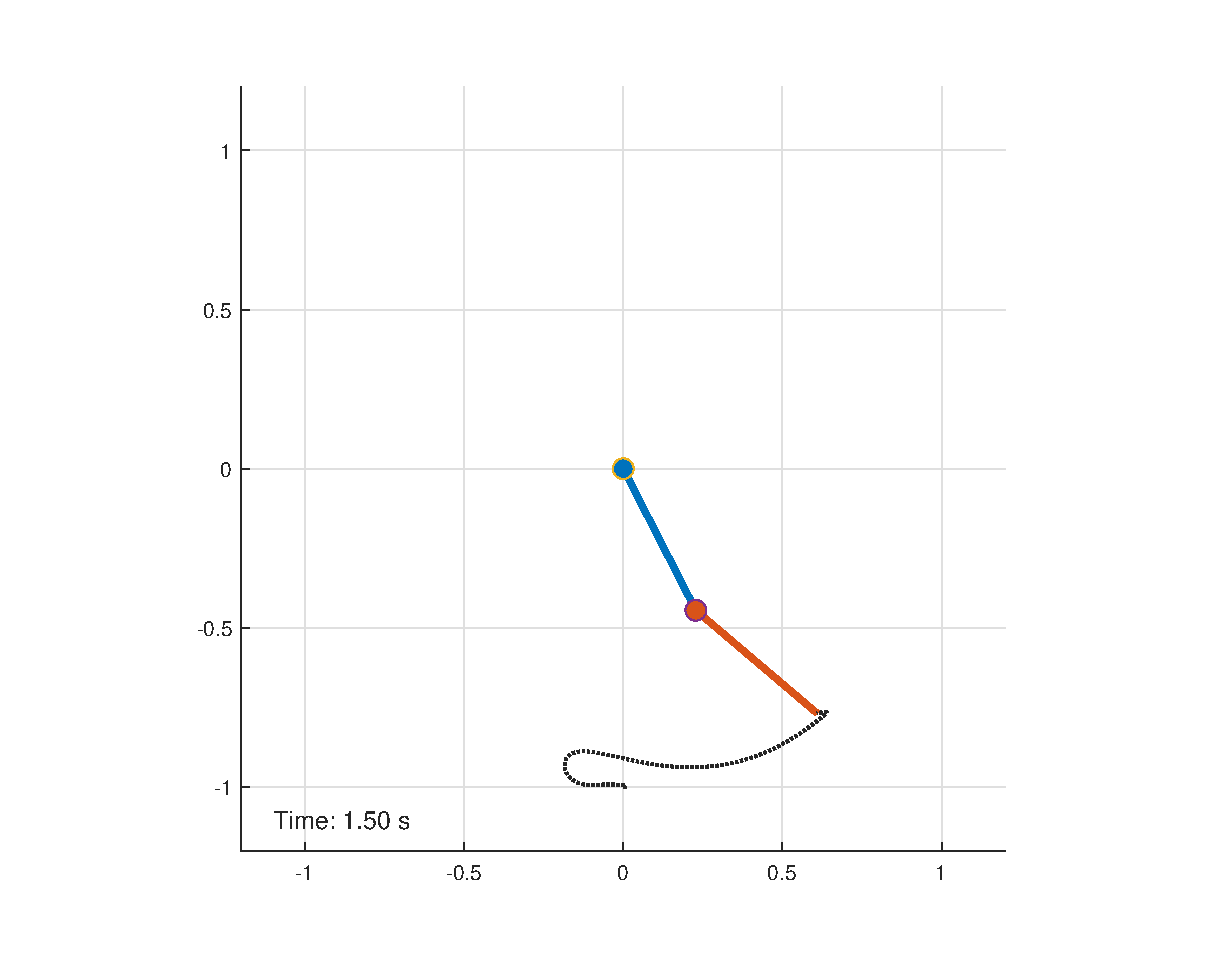
\includegraphics[width=0.25\textwidth,trim={3cm 1cm 1cm 1cm},clip]{assets/pendubot_qp_anim_2.eps} \hspace*{-0.5cm}
    \includegraphics[width=0.25\textwidth,trim={3cm 1cm 1cm 1cm},clip]{assets/pendubot_qp_anim_3.eps} \hspace*{-0.5cm}
    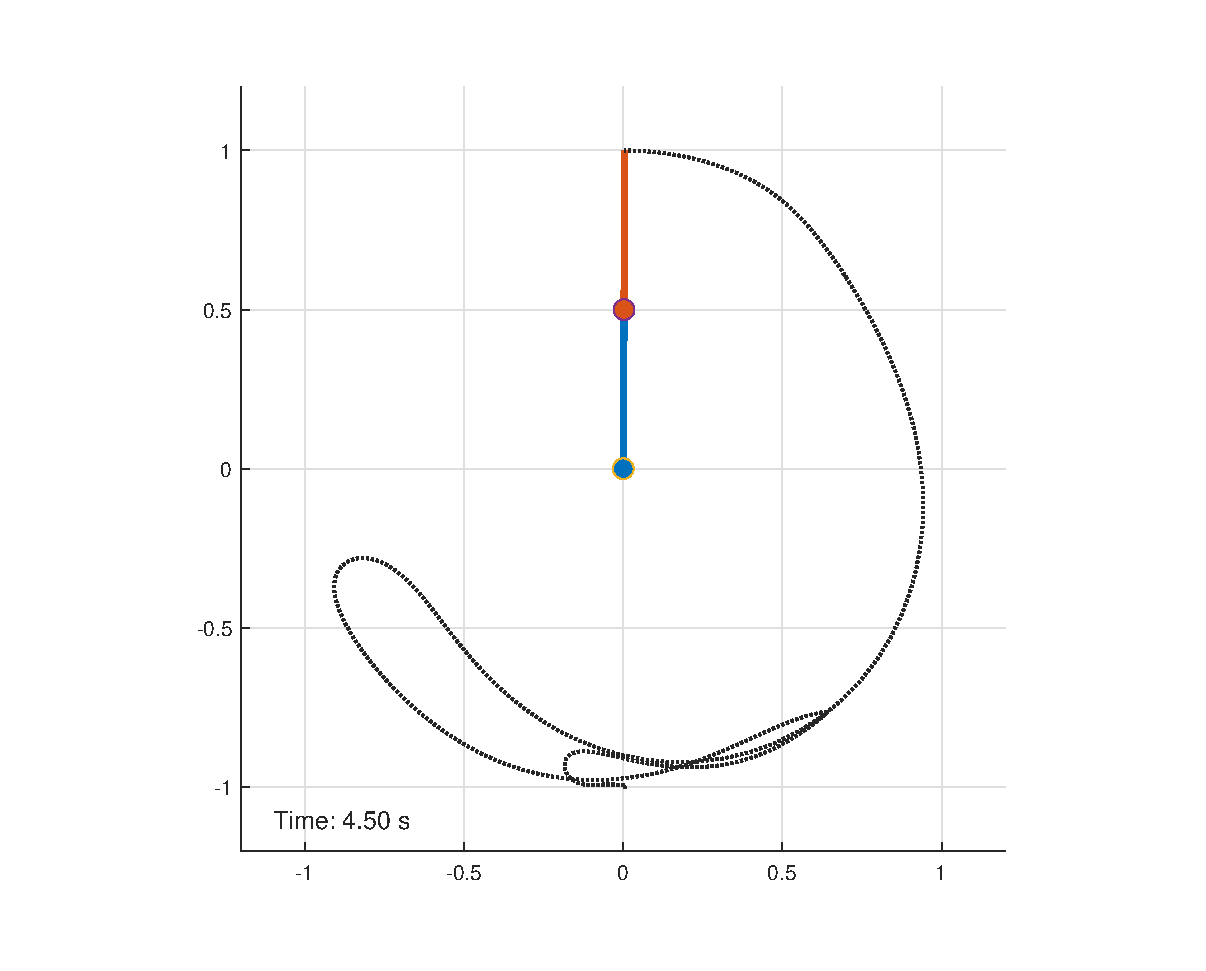
\includegraphics[width=0.25\textwidth,trim={3cm 1cm 1cm 1cm},clip]{assets/pendubot_qp_anim_4.eps}
    \caption{Animation frames of the pendubot swing-up motion under constrained quadratic programming.}
    \label{fig:pendubot_anim}
\end{figure}
\begin{multicols}{2}

\subsubsection{Acrobot}
Conversely, the model of the acrobot is retreived by not actuating the first joint of the robot in Figure \ref{fig:robot}, i.e., by setting $u_1$ identically equal to zero. This time, the limits imposed on the actuated joint are $u_{\text{min}} = -\SI{3.5}{\newton\meter}$ and $u_{\text{max}} = \SI{3.5}{\newton\meter}$, which are less restrictive than the previous case due to the different physical properties of the robot.

Just as it was done for the pendubot, the trajectories of the acrobot under the three different constraining strategies are depicted in Figure \ref{fig:acrobot_traj}, and the animation of the swing-up motion under constrained quadratic programming is shown in Figure \ref{fig:acrobot_anim}. The results are consistent with the previous expreriments, as the constrained quadratic programming method is the only one able to perform the swing-up motion, besides the case with no constraints. In addition to this, note the fact that, when employing naive clamping or the squashing function, the control sequences are similar to each other, are not too close to the extremes of the admissibility interval, and yet are unable to achieve the intended goal: evidently, the constraining methods have penalized the search for the optimal solution during the controller iterations, reflecting the disadvantages that were pointed out in the related section.

\end{multicols}
\begin{figure}[H]
    \centering
    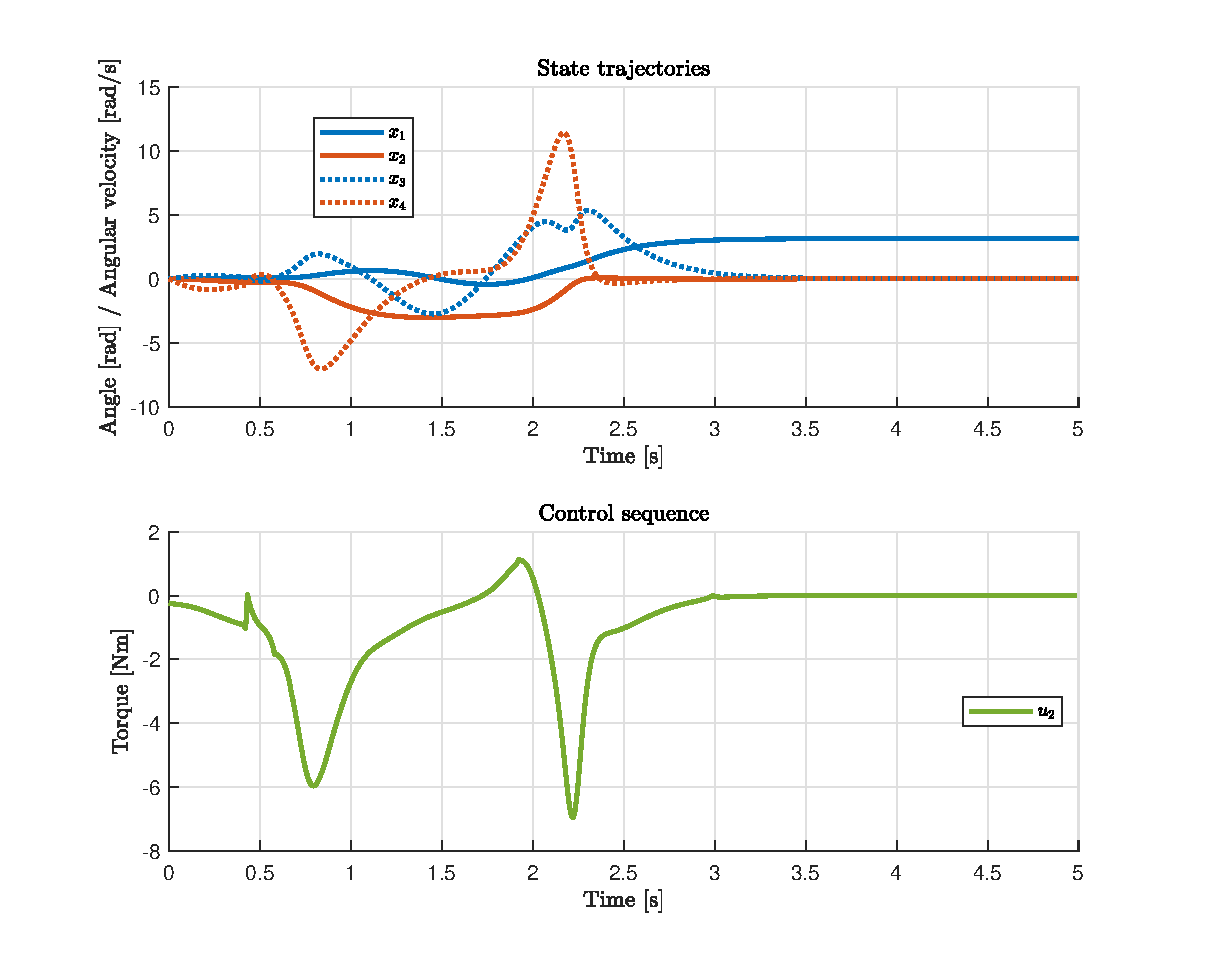
\includegraphics[width=0.4\textwidth]{assets/acrobot_traj.eps}
    \includegraphics[width=0.4\textwidth]{assets/acrobot_nc_traj.eps} \\
    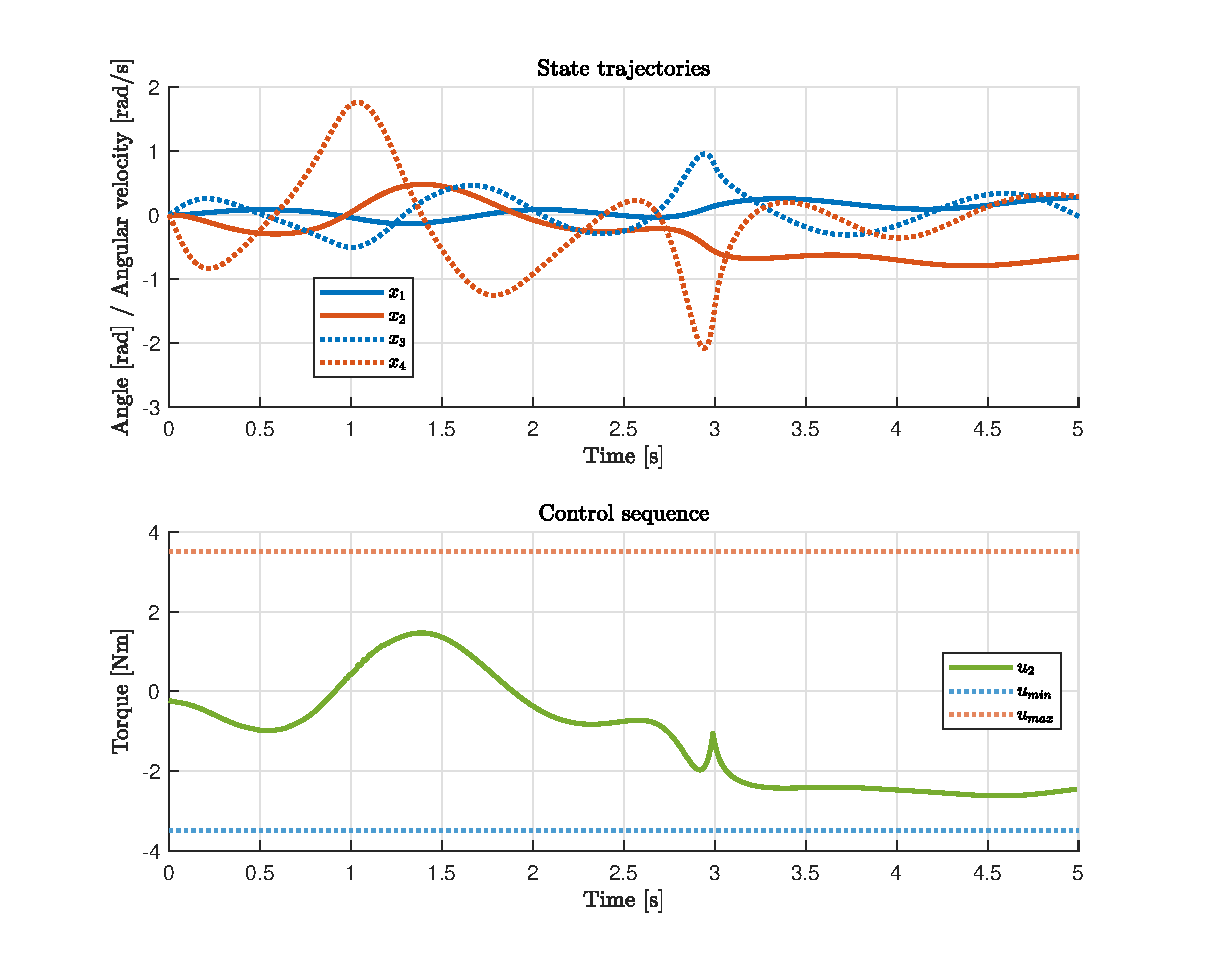
\includegraphics[width=0.4\textwidth]{assets/acrobot_sf_traj.eps}
    \includegraphics[width=0.4\textwidth]{assets/acrobot_qp_traj.eps}
    \caption{Trajectories of the acrobot under: no constraints (top left), naive clamping (top right), squashing function (bottom left), constrained quadratic programming (bottom right).}
    \label{fig:acrobot_traj}
\end{figure}

\begin{figure}[H]
    \centering
    \includegraphics[width=0.25\textwidth,trim={3cm 1cm 1cm 1cm},clip]{assets/acrobot_qp_anim_1.eps} \hspace*{-0.5cm}
    \includegraphics[width=0.25\textwidth,trim={3cm 1cm 1cm 1cm},clip]{assets/acrobot_qp_anim_2.eps} \hspace*{-0.5cm}
    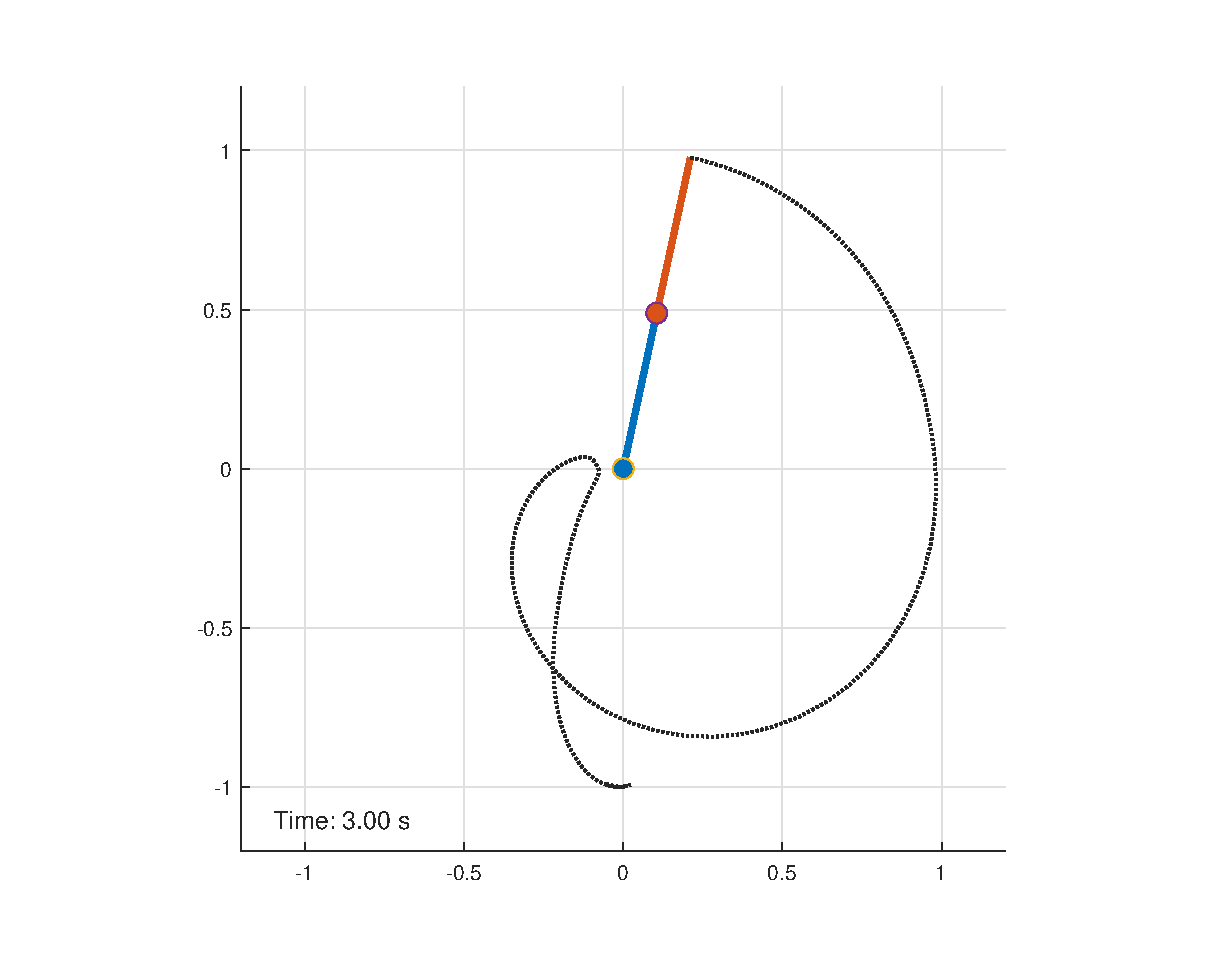
\includegraphics[width=0.25\textwidth,trim={3cm 1cm 1cm 1cm},clip]{assets/acrobot_qp_anim_3.eps} \hspace*{-0.5cm}
    \includegraphics[width=0.25\textwidth,trim={3cm 1cm 1cm 1cm},clip]{assets/acrobot_qp_anim_4.eps}
    \caption{Animation frames of the acrobot swing-up motion under constrained quadratic programming.}
    \label{fig:acrobot_anim}
\end{figure}
\begin{multicols}{2}